%%%%%%%%%%%%%%%%%%%% author.tex %%%%%%%%%%%%%%%%%%%%%%%%%%%%%%%%%%%
%
% sample root file for your "contribution" to a contributed volume
%
% Use this file as a template for your own input.
%
%%%%%%%%%%%%%%%% Springer %%%%%%%%%%%%%%%%%%%%%%%%%%%%%%%%%%%%%%%%%


%% RECOMMENDED %%%%%%%%%%%%%%%%%%%%%%%%%%%%%%%%%%%%%%%%%%%%%%%%%%%
%\documentclass[graybox]{svmult}
%
%% choose options for [] as required from the list
%% in the Reference Guide
%
%\usepackage{mathptmx}       % selects Times Roman as basic font
%\usepackage{helvet}         % selects Helvetica as sans-serif font
%\usepackage{courier}        % selects Courier as typewriter font
%\usepackage{type1cm}        % activate if the above 3 fonts are
                             % not available on your system
%
%\usepackage{makeidx}         % allows index generation
%\usepackage{graphicx}        % standard LaTeX graphics tool
%                             % when including figure files
%\usepackage{multicol}        % used for the two-column index
%\usepackage[bottom]{footmisc}% places footnotes at page bottom
%
%% see the list of further useful packages
%% in the Reference Guide
%
%\makeindex             % used for the subject index
%                       % please use the style svind.ist with
%                       % your makeindex program
%
%%%%%%%%%%%%%%%%%%%%%%%%%%%%%%%%%%%%%%%%%%%%%%%%%%%%%%%%%%%%%%%%%%%%%%%%%%%%%%%%%%%%%%%%%%
%
%\begin{document}

\title{Infrastructure Systems}
% Use \titlerunning{Short Title} for an abbreviated version of
% your contribution title if the original one is too long
\author{
    \textbf{Rodrigo Costa}
    \and Rodrigo Silva-Lopez 
    \and Luis Ceferino 
    \and{Vesna Terzic}
    \and{Ann-Margaret Esnard}
    \and{Henry Burton}}
\tocauthor{}
\authorrunning{Costa et al.}
% Use \authorrunning{Short Title} for an abbreviated version of
% your contribution title if the original one is too long
%\institute{Name of First Author \at Name, Address of Institute, %\email{name@email.address}
%\and Name of Second Author \at Name, Address of Institute %\email{name@email.address}}
%
% Use the package "url.sty" to avoid
% problems with special characters
% used in your e-mail or web address
%
\maketitle
Critical infrastructure is the term used to describe systems and assets which if incapacitated or destroyed would have a debilitating effect on security, national economic security, national public health or safety, or any combination thereof \citep{DHS_CI}. These report focuses on critical infrastructure in the transportation, water, wastewater, power, fuel, health systems. In comparison to recovery of housing or business, the modeling of disaster recovery for individual critical infrastructure system has been more extensively investigated. However, critical infrastructure systems are dependent on each other, with failures to one system being potentially propagated to others. More comprehensive studies of system interdependence, cascading failures, and its impact on society are still needed to foster community resilience. This review introduces some key concepts on the modeling of critical infrastructure systems, first at a broader level, followed by a discussion of specific points regarding different systems.\ 

\FloatBarrier
% -----------------------
\section{Input and Output Data}
% -----------------------
Modeling the recovery of critical infrastructure systems requires estimates of the time needed to repair each component (including facilities) in these systems. This topic is discussed in detail in Part \ref{part:Performance}. Beyond repair time estimates, it is necessary understand the interdependencies between these components, as well as the interdependencies with other systems. Reports by local authorities are the primary source of publicly available information for critical infrastructure systems. These provide information on the location, characteristics, and connections of the components, which can used for simplified analyses. However, detailed analysis, e.g., hydraulic models of water systems, are often reliant on information from private entities that can only be obtained through agreements with system operators. Beyond that, operators of a system are rarely aware of how other systems are reliant on the system they operate. Due to this siloed management, there is no one organization that can provide comprehensive information on the interdependencies of the system they operate. This is one of the main challenges to the development of comprehensive and integrated models for critical infrastructure recovery.\ 

%\FloatBarrier
% -----------------------
\section{Concepts in Critical Infrastructure Modeling}
% -----------------------
Critical infrastructure systems comprise components and their connections, be those physical or not. These connections cause the disruption of certain components to have cascading effects on the whole system \citep{rinaldi2001identifying}. For this reason, the modeling of critical infrastructure interdependence has gained much attention in the last two decades and several modelings techniques have been used for this purpose. \cite{Eusgeld2008a} reviewed almost 100 articles on modeling of interdependent infrastructure systems published between 1987 and 2007, identifying eight modeling techniques: (1) agent-based modeling, (2) system dynamics modeling, (3) hybrid system, (4) input-output-model, (5) hierarchical holographic modeling, (6) critical path method, (7) high-level architecture, and (8) Petri nets. In a more recent review of nearly 200 articles, \cite{ouyang2014review} defines five main groups of modeling techniques: (1) empirical approaches, (2) agent-based approaches, (3) system dynamics models, (4) economic theory-based approaches, and (5) network-based approaches. \cite{ouyang2014review} compared these techniques regarding their applicability to evaluate resilience-improving strategies. Agent-based and network flow-based models were able to support the most resilience improvement strategies. The readers are referred to the review papers by \cite{Eusgeld2008a} and \cite{ouyang2014review} for descriptions of these techniques, including their strengths and limitations. \ 

Beyond interdependence within a system, critical systems may also be dependent on each other, creating a system of systems, as discussed in the seminal paper by \cite{rinaldi2001identifying}. If recovery of interdependent systems is of interest, a decision about the modeling approach is necessary. Two alternatives are illustrated in Figure \ref{fig:Interdependencies}. On the left-hand side, a multi-layer approach is shown. In this approach each system can be simulated independently \citep{guidotti2017multi}. The results of the analyses of the upper systems are inputs to the lower systems. The main advantage of this approach is that each system can be simulated using a different technique and level of detail. \cite[p.243]{cimellaro2016resilience} provides a detailed description of the multi-layer approach. On the right-hand side, a single-layer approach is shown. In this approach, all systems are simulated simultaneously and one simulation technique has to be used throughout. These limitations are offset by the capacity of this approach to simulate interdependence between facilities, rather than systems. For example, a single-layer approach can simulate the interdependence between a power substation and a water pump station, as well between a water pump station and a power generation facility, in the same time step. This is not possible with a multi-layer approach.\ 

\begin{figure}[htb]
    \centering
    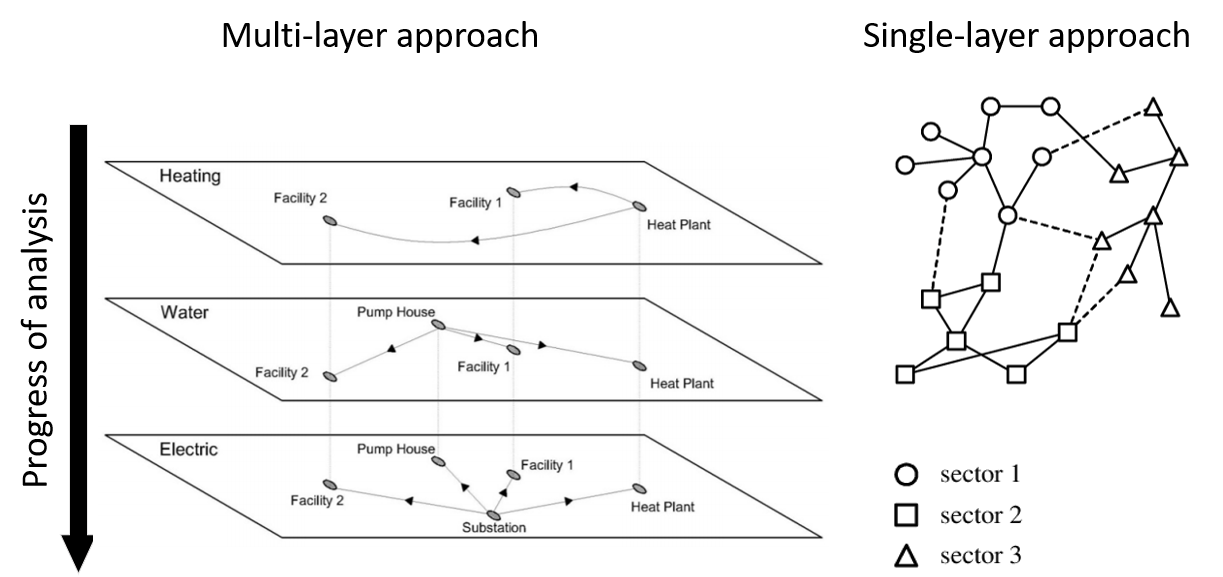
\includegraphics[width=0.8\textwidth, angle = 0]{Figures/Interdependencies.png}
    \caption{Approaches to interdependency modeling (adapted from \cite{cimellaro2016resilience}).}
    \label{fig:Interdependencies}
\end{figure}

%\FloatBarrier
% -----------------------
\subsection{Land transportation systems}
% -----------------------
Transportation network disruption due to natural hazards has shown to generate significant impacts on communities' ability to recover. Traffic disruption following the collapse of bridges and roads can affect businesses long after the triggering event \citep{boarnet1998business}. Also, it has been observed that downtime of transportation systems affects the long-term recovery of regional economies \citep{chang2000transportation}. Taking that into account, the recovery of these systems is an important aspect to incorporate when modeling urban resilience. \

The recovery of transportation systems imposes several challenges derived from the inherent complexities of these networks: The interdependencies between bridges are highly non-linear, and modeling how people will travel has proven to be difficult, especially after natural disasters \citep{chang2010transportation}. As the first step to model recovery, several studies have attempted to estimate repair time for bridges and roads through the development and implementation of restoration curves \cite{HAZUS-MH2015,padgett2007bridge}. While these curves are fundamental to assess the recovery of transportation systems, it is necessary to develop models that account for the network interactions of roads, bridges, and traffic demand. It is in that regard that researchers have developed different strategies to help decision-makers to manage transportation assets for enhanced recovery. One strategy has been to develop optimized scheduling of bridge repairs. This approach aims to propose the order in which bridges should be repaired or restored, so travel flow in the region recovers to its previous level in the shortest time \citep{vugrin2014optimal}. Besides focusing on the flow of the network, some studies have explored how resources, funds, and crews, should be allocated \citep{karlaftis2007fund}. A second strategy explored has been to propose retrofitting actions, which instead of making the recovery time shorter, decrease the initial network disruption \citep{zhang2016resilience}. These two strategies are complementary and can often be implemented synergistically.\ 

%\FloatBarrier
% -----------------------
\subsection{Power systems}
% -----------------------
The timely recovery of electric power systems is particularly critical because most other lifeline systems need electricity for their operation and management. Recovery for power systems is often measured by the amount of flow or services delivered, the availability of power for critical facilities, the number of customer served, or the support of economic activities. Although power system are comprised of several components, e.g. transformers, and switches, it may be impractical to include all in a model. Typical critical facilities of electric power systems include generation power plants and transmission substations that are connected by transmission and distribution lines. The transmission lines connect generation power plants to transmission substations which carry high voltage electricity over long distances. Additionally, distribution lines, carrying lower voltage electricity, deliver electricity to end users. \

Modeling of post-disaster recovery of electrical power systems has been approached by using statistical and simulation-based models. Statistical approaches are easier to implement and require less computational power. However, these approaches require significant amount of training data and cannot be used for ``what-if'' analyses, which are important for recovery planning. A review of statistical based model is provided by \cite{liu2007statistical}. The authors collected data on the duration of power shortages at different locations after Hurricane Ivan in 2004. A 10-fold cross validation method was employed and the out-of-sample error was calculated and compared to a naive model defined simply as the mean power shortage duration. Five methods were investigated: (i) accelerated failure time (AFT), (ii) Cox proportional hazard models (Cox PH), (iii) regression trees (CART), (iv) Bayesian additive regression trees (BART), and (v) multivariate additive regression splines (MARS). The BART, MARS, and AFT approaches presented improved prediction capacity when compared to the naive model, whereas the Cox PH and CART did not present an improvement over the naive model. \ 

Among the simulation-based approaches, those based on arcs and nodes, as well as discrete-event simulation, and agent-based approaches are the most common \citep{Eusgeld2008a,ouyang2014review,sun2019resilience}. In these approaches the components of the system are modeled explicitly and their post-disaster state is evaluated using fragility curves. The availability of resources and the sequence of restoration are also modeled \citep{ouyang2014multi}. The main advantage of these approaches is their ability to consider the effects of different strategies, e.g., different restoration sequences, to support resilience. This disadvantage is that they require detailed information about the system, which may not be publicly available. \ 

%\FloatBarrier
% -----------------------
\subsection{Water and wastewater systems}
% -----------------------
Disruptions to water and wastewater systems can exacerbate the impacts of disaster by compounding sanitary and ecological issues. Moreover, households and businesses in physically safe buildings may be forced to leave or not operate due to interruptions in water and wastewater services. These reasons make water and wastewater systems pivotal for recovery.\

Infrastructure involved in water delivery and wastewater collection include pumping stations, treatment and purification stations, reservoirs, storage tanks or towers, as well as water pipelines. Another consideration relevant to water and wastewater system is the post-disaster capacity of the system. Water stored in distribution tanks may provide residual capacity to serve customers during recovery. However, comprehensive studies of storage tanks subjected to earthquake loads have shown that there is correlation between the tank fill level and physical vulnerability \citep{orourke2000seismic, eidinger2012recent, cooper1997study}. For wastewater systems, if their post-disaster capacity is significantly compromised, the system may overflow some time after the event. In both cases, it is important for recovery models to account for the demand for these systems during recovery.\

Water and wastewater systems have been studied using several modeling approaches. \cite{miles2019community} separate these into seven groups: resource-constrained modeling, machine learning, network modeling, system dynamics, agent-based, discrete-event, and stochastic simulation. A review of these techniques, their advantages and limitations are discussed in detail in \cite{miles2019community} and not replicated here for brevity. The choice between these approaches is influenced by the recovery metric being used. For example, machine learning algorithm excel in estimating the duration of probable disruptions but offer limited guidance for the operational management especially in the case of insufficient data. Agent-based and discrete event simulations do not share this limitation, however, may require significant effort to simulate the flow relevant characteristics of various components. Network-based approaches can represent flow well, but if overly-abstracted can result in erroneous conclusions and lead to ineffective allocation of resources \citep{Hines2010a}. \

%\FloatBarrier
% -----------------------
\subsection{Fuel systems}
% -----------------------
Fuel shortages in the aftermath of disasters are not uncommon \citep{Smythe2013, Holguin-Veras2014}. These disruptions can cause logistical as well as public relations concerns, compound emergency response difficulties, and affect public services. The reality however is that no one entity has control over this system. Fuel caches are stored at gas stations and local authorities may have difficulty controlling the distribution of fuel. Additionally, panic-buying, or hoarding, is a common practice after extreme events \citep{shen2017development, helbing2006disasters}, and the demand for fuel may significantly increase following a disaster. These characteristics make the simulation of the recovery of fuel systems reliant on a deep understanding of the system and community at hand. \

Two approaches exist in the literature to simulate hoarding behavior. The economic theory assumes that consumers are rational individuals that seek to maximize their utility. Thus, models based on utility theory are good candidates to simulate hoarding from the economic theory perspective. Game theory \citep{hallsworth2000urban}, and the ``Tragedy of the Commons'' \citep{hardin2009tragedy} fall in this category. The assumption of perfect rationality is appealing because it simplifies the models. However, other scholar challenge this assumption and view consumers individuals with bounded rationality, imperfect information, and limited cognitive ability and time to make decisions. A comprehensive discussion on the bounded-rationality theory is provided by \cite{sep-bounded-rationality}. \

%\FloatBarrier
% -----------------------
\subsection{Hospital systems}
% -----------------------
Hospitals are critical in the aftermath of a disaster because they must respond to the emergency by treating patients and preventing additional deaths. Disasters can place particularly high strains on hospitals because they can cause injuries as a result of damage to infrastructure \citep{ceferino2018regional,ceferino2018probabilistic,johnston20142010,jun2010analysis}. Additionally, natural disasters can dramatically reduce the hospitals' ability to function. Damage to a hospital's structural and non-structural components can rapidly disrupt the functionality of treatment procedures highly necessary for earthquake patients \citep{bambaren2011a3,mitrani2012functional}. The recovery of hospital systems is particularly dependent on other infrastructure systems. Hospitals dependent on utilities such as power and water to operate \citep{Chand2015, jacques2014resilience, Achour2014, Hiete2011, McDaniels2008}; on fuel for ambulances and power generation if electrical power is disrupted \citep{Hiete2011}; and on the transportation network for accessibility. Organizational challenges, e.g., limited staff, are another issue for the recovery Hospital systems \citep{Cimellaro2016}. \

The literature suggests using the quality of the healthcare provided as a metric of recovery \citep{vieth2006effect, hamby2004using}. The waiting time that a patient needing assistance spends in the queue before receiving it is often used as a proxy of the quality of the medical care. Methods to model hospital response after disasters have been developed mainly at the single-hospital scale. Structural modeling and functionality models have been key to evaluating the hospital ability to provide treatment after disasters \citep{cimellaro2011performance,jacques2014resilience,yavari2010modeling}. Other methods based on discrete event simulation and minimum-cost flow models have been developed to represent emergency response and allocate resources during the earthquake aftermath but also at the single-hospital scale \citep{aghapour2019capacity,gul2015comprehensive,vugrin2015modeling,yi2005real}. More recently, a model on emergency response of hospitals at the system-scale rather than at the single-hospital scale was proposed \citep{ceferino2019effective}. The higher complexity and data requirements of this approach are offset by its ability to simulate coordination between hospitals to effectively allocate medical resources and patients. This coordination is key to guarantee patients are treated timely after disasters.\

% -----------------------
\section{Major Research Gaps and Needs}
% -----------------------
While the modeling of individual critical infrastructure system recovery has progressed significantly, the modeling of the recovery of interdependent systems requires further research. To foster community resilience, it is fundamental to understand how the recovery of each system relies on other systems and how this affects the recovery of businesses and households. This effort will require solid collaborations between researchers and the public and private sectors, due to privacy concerns regarding the data needed for the development of these models. Recent studies have also demonstrated that hindcasting can be effectively used to validate the recovery of individual infrastructure systems \citep{tomar2020hindcasting}. Model validation via hindcasting, as well as the collection of data to support hindcasting are topics that require further research. \

\FloatBarrier